\documentclass[12pt,a4paper]{article}
\usepackage{amsmath}
\usepackage[T1]{fontenc}
\usepackage[utf8]{inputenc}
\usepackage{setspace}
\onehalfspacing
\usepackage{graphicx}
\usepackage{subcaption}
\usepackage{pst-tree}
\usepackage{tikz}
\usetikzlibrary{trees}
\usepackage{amsfonts}
\usepackage{amsthm}
\usepackage[top=2.5cm, bottom=2.5cm, left=2.5cm, right=2.5cm]{geometry}
\usepackage{enumerate} 
\usepackage{amssymb}
\usepackage{csquotes}
\usepackage{fancyhdr}
\usepackage{times}
\usepackage{fancyhdr}
\usepackage[bottom]{footmisc}
\pagestyle{fancy}
\usepackage{amsmath}
\usepackage{amssymb}
\usepackage{graphicx}
\usepackage{tikz}
\usepackage{lscape}
\newcommand*\circled[1]{\tikz[baseline=(char.base)]{
\node[shape=circle,draw,inner sep=2pt] (char) {#1};}}
\DeclareMathSizes{12}{12}{10}{10}
\interfootnotelinepenalty=10000
\usepackage{dsfont}
\usepackage{mathtools}
\usepackage{graphics}
\usepackage{graphicx}
\usepackage{multirow, booktabs}
\usepackage[final]{pdfpages}
\usepackage{hyperref}
\usepackage{xcolor}
\usepackage{booktabs,siunitx}
\usepackage{float}
\usepackage{caption}
\usepackage{footnote}
\makesavenoteenv{tabular}
\usepackage{tablefootnote}
\lhead{}
\rhead{}
\chead{Social Data Science, Summer 2019.}


\begin{document}
\includepdf[pages=-]{forside.pdf}
\newpage
\onehalfspacing

\tableofcontents
\newpage
\section{Introduction}
This report depicts a research performed regarding active Danish real estate property valuations. Since 2011, the annual number of real estate properties sold has slightly increased, with 2017 being the year with most sold properties in 10 years \href{https://www.dst.dk/da/Statistik/nyt/NytHtml?cid=27979}{(Danmarks Statistik, 2018)}. The price of real estate properties is also rising through 2019 \href{https://www.dst.dk/da/Statistik/nyt/NytHtml?cid=28741}{(Danmarks Statistik, 2019)}. Although this generally depicts a willingness of buyers to pay more for real estate property, and higher valuations from realtors, a closer analysis of active valuations adds a local view of which conditions contribute to the valuation of a real estate property. \newline
\newcommand{\source}[1]{\caption*{Source: {#1}} }\begin{figure}[H]
\centering
\caption{}
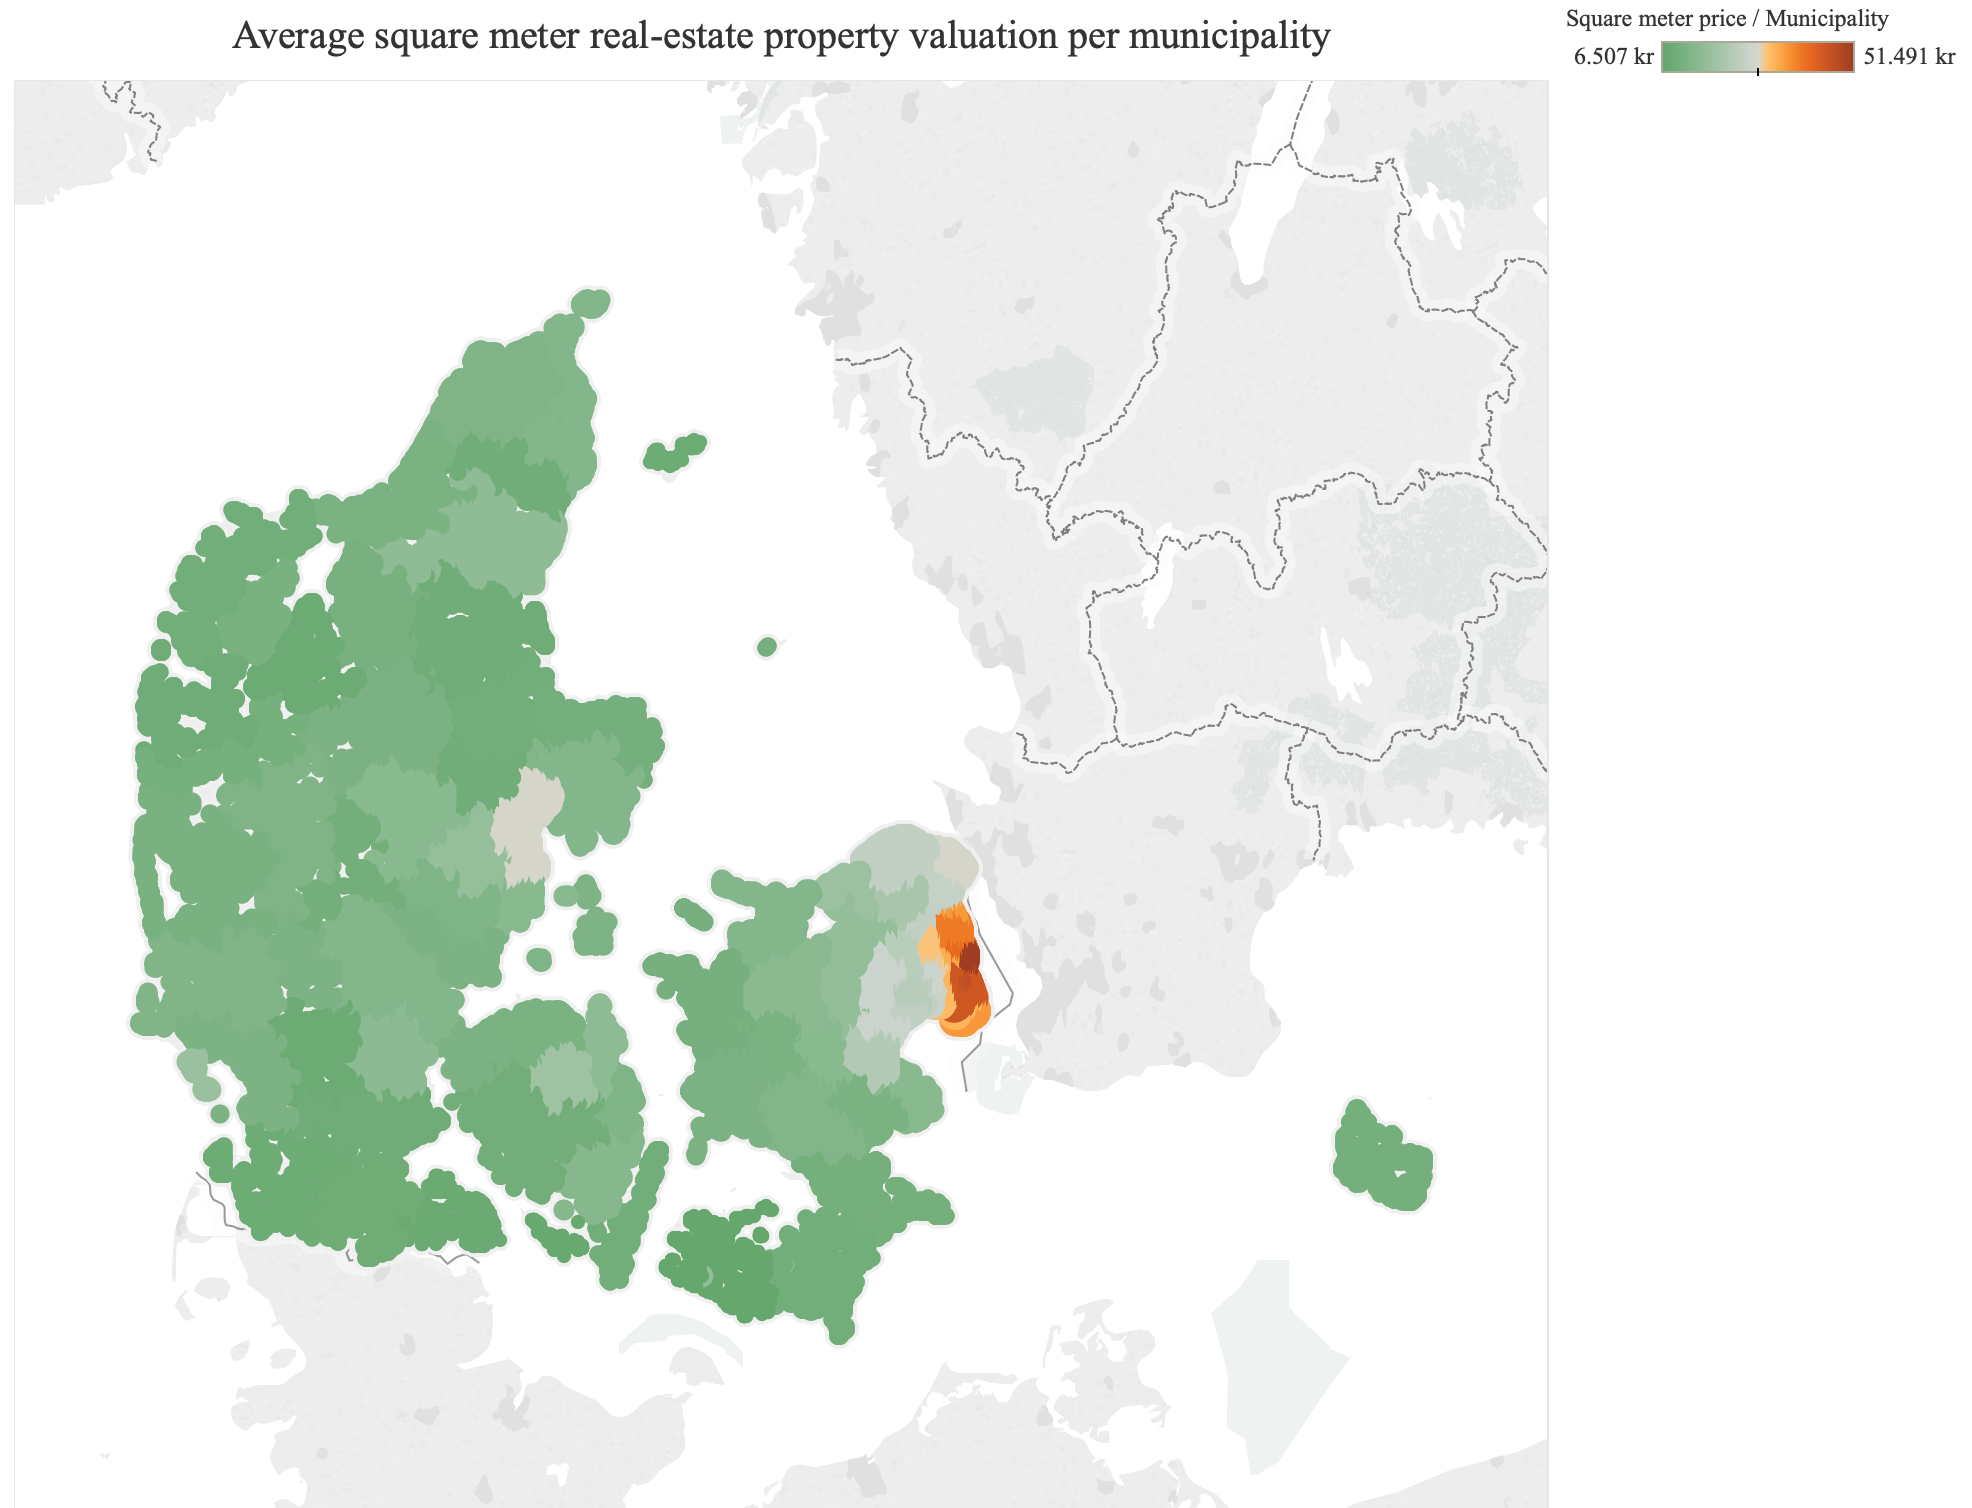
\includegraphics[scale=0.4]{123.png}
\source{Own creation, with data from \href{https://www.boliga.dk}{Boliga.dk}}
\end{figure}

Figure 1 shows the average square meter price valuation of active offers per municipality in Denmark. The maximum square meter price being approximately 8 times higher in the municipality of Gentofte, than Lolland, the municipality with the lowest average square meter price valuations. A tendency visualised in the figure, is that average square meter price valuations are higher in highly populated municipalities and in suburban areas surrounding Copenhagen. \newline

The valuations included in the research are collected from one of Denmarks largest online real estate websites named Boliga.dk. The Boliga data contains approximately 66,000 active offerings with valuations ranging from DKK 15,000 to DKK 85 million. This research paper intends to analyse real estate price valuations and which geo- and sociodemographic criteria affect valuations, using machine learning models. Our research question is as follows: 
\begin{center}
 \textit{Which features are most relevant for predicting valuations of real estate properties in Denmark?}
\end{center}
This research paper contains a section describing the construction of research data and assesses the choices made in gathering meaningful features for the dataset. Also, a section regarding the choice and optimization of machine learning models is included, where the intention is to provide insights on our progress of finding the optimal model. As a result, the best performing model is chosen with a discussion of its usability. 

\section{Literature Review}
Within social data science there exist widely differing definitions of big data and machine learning. This section seeks to clarify the use of these terms within the scope of this paper.
\subsection{On Big Data \& Machine Learning}
Historically, big data has been a term reserved for data that was unable to be processed by extant software. However, recent increases in computational power has enabled data processing of hitherto unheard of quantities of data\footnote{Lazer, David and Jason Radford (2017) \textit{Data ex Machina. Introduction to Big Data}. Annual Review of Sociology}. Today, big data is no longer too cumbersome to analyse. Matthew Salganik\footnote{Salganik, Matthew J. (2018) \textit{Bit by Bit Bit - Social research in the digital age.}} instead mentions ten typical characteristics of big data. Salganik's tentative definition suggests that big data is not a single entity, but includes many different types of systems. Among the most important features of Salganik's definition of big data is that the data has a high frequency of observations and is continuously being generated. Since the data is always-on it is also drifting, meaning that the structure and population it represents is ever-changing. It is therefore important to understand that big data is not a naturally occurring system, but driven by the engineered purpose of the system. This algorithmic confounding force the scientist to be careful regarding any observed human behaviour that is extracted from a single digital system.\newline
In the analysis of big data it is often useful to employ machine learning as it can identify and predict various non-linear relationships in big data sets, that otherwise would remain hidden. Data scientists' have for the most part optimised the predictive capabilities of the algorithm applied, and as a consequence they have often ignored or trivialised machine learning's potential in causal modelling\footnote{Varian. Hal R. \textit{Big data: New tricks for econometrics}}.\newline
The technical and theoretical challenges faced by big data and machine learning research are important to consider, when employing the tools they provide. One of the major discussions revolve around machine learning's predictive capabilities. Chris Anderson\footnote{Anderson, Chris. (2008), \textit{The end of theory: The data deluge makes the scientific method obsolete}} argues that since the computing power and the scale of data has increased exponentially, our reliance on scientific models could become obsolete. Instead of focusing on the theoretical implications of observations, scientists should, according to Anderson, focus on the statistical outputs: In the age of big data, correlation perhaps should supersede causality and consequently social data scientists should not try to develop coherent models or unified theories to explain a social phenomenon.\newline
However, many social data scientists argue against this point of view. Justin Grimmer\footnote{Grimmer, Justin (2015) \textit{We are all social scientists now: how big data, machine learning, and causal inference work together}} claims, that correlations extracted from big data cannot stand alone. Large quantities of data is not sufficient to make scientifically valid causal inferences. It requires a rigorous research design and clear theoretical assumptions, in order to yield scientifically accurate estimates. Indeed the social sciences greatest contribution to big data research, comes from the organised framework provided by rigorously tested theory\footnote{Einav, Liran and Jonathan Levin (2014) \textit{Economics in the age of big data}}.\newline
The contribution from the social sciences to machine learning help create new methods that will be able to utilise the strengths of machine learning to help solve causal inference problems within the framework of a well defined theory\footnote{Athey, Susan (2018) 'The Impact of Machine Learning on Economics' in Ajay Agrawal et al. (eds) \textit{The Economics of Artificial Intelligence: An Agenda}}. These new approaches could help define what variables to manipulate and how to properly use machine learning within the framework of theoretical assumptions. Ultimately, big data and machine learning could increase the scope of the social scientist's field, not only by delivering new data and methods, but by helping the social scientist to focus on new questions\footnote{Mullainathan, Sendhil, and Jann Spiess (2017) \textit{Machine Learning: An Applied Econometric Approach}}.

\subsection{An Ethical Overview}
The ethical principles of social research are anchored in the fundamental human rights, which are broadly formulated in the UN Declaration of Human Rights. Additional policies and declarations that codify principles of research ethics and the ethical treatment of research participants include the Nuremberg Code, the Helsinki Declaration, the Belmont Report, and the Menlo Report\footnote{Salganik, Matthew J. (2018) \textit{Bit by Bit Bit - Social research in the digital age.}}\, \footnote{European Commission (2018). \textit{Ethics in Social Sciences and the Humanities}}. These codes and addendums originate mostly in the biomedical field, though they encompass the central principles applied to all human research, which have led some academics to call for a Hippocratic oath for data scientists to safeguard against powerful new technologies under development in laboratories and tech firms\footnote{Rotblat, Joseph (1999) \textit{A Hippocratic Oath for Scientists}}\, \footnote{Sample, Ian (2019, Fri 16 Aug 2019) \textit{and tech specialists need Hippocratic oath, says academic.}}. This discussion is nothing new however, as a tentative reformulation of the Hippocratic oath was introduced by Karl Popper\footnote{Popper, Karl (1969) \textit{The Moral Responsibility of the Scientist}}, wherein he stressed the importance of professional responsibility, a critical mind, and an overriding loyalty towards the betterment of mankind.\newline
Matthew Salganik offer four principles deduced from the Belmont and Menlo Report that should guide the ethical deliberations of the researcher: 1) the respect for persons, that is individuals should be treated as autonomous and if circumstances require it individuals should be entitled to additional protections. 2) Beneficence stresses the importance of doing no harm and to maximise the possible benefits and minimising any potential harms. 3) The principle of justice touches upon the importance of the distribution of burdens and benefits of the social scientist's research. This principle stress that is should not be a single stratum of society that bears the costs of the research while another stratum benefits. 4) The fourth and final principle is the respect for law and public interest, according to Salganik, the principle consists of two distinct elements, that is compliance to relevant laws and legal contracts and transparency-based accountability. It is worth noting that Popper’s tentative Hippocratic oath mirrors the first three principles put forth by Salganik, stressing the importance of the ethical conduct of the researcher.\newline
The need for rigid ethical standards within computational social science was made apparent by the Cambridge Analytica Scandal that broke on the 17th of March 2018. Where Steve Bannon could reveal that between 2013 and 2015 Cambridge Analytica had exploited a loophole in Facebook’s API which allowed the company to harvest profile data from 87 million Facebook users, without the user’s permission and use the harvested data to construct a massive targeted marketing database based on the user’s likes and interests\footnote{Vox.com (2018) \textit{The Cambridge Analytica Facebook scandal} [Online]}. Other examples of misuse of data acquired from Facebook include the Harvard-run experiment, where students' data was used to create new knowledge about how social networks form and how these networks and their actors' behavior co-evolve, and the emotional contagion experiment from 2012, where approximately 700,000 users were involved in a research experiment to examine the extent to which a person's emotions are affected by the emotions of the people they interact with (Salganik. 2018).\newline
From this it should be evident that clear ethical guidelines are required in order to protect the user's privacy from tech-savvy companies. To this end, the European Parliament introduced the General Data Protection Regulation (GDPR). With its seven overarching principles the GDPR seeks to formalise the procedures involved in the data processing and storing of sensitive and private information (CDRC\footnote{Consumer Data Research Center, UK  [CDRC] (2018) \textit{The General Data Protection Regulation \& Social Science Research} [Online]:}). These principles include and expand upon the principles found in the Belmont and Menlo Report. The most important consideration, however, must be that even a dataset comprising tens of thousands of observations involve human beings who must be protected from adverse side-effects of the social research. There is considerable evidence that point to the fact that even in anonymised data sets it can be possible to backtrack an individual's identity. A researcher must therefore be mindful of the mosaic effect if the dataset combines large amount of data from various sources (European Commission 2018).

\section{Data Description \& Ethics}

\subsection{Ethical Considerations in the Current Research Project}
In the current paper the appropriate care and consideration has been given to the ethical concerns regarding the scraping, processing, and the presentation of the data. Drawing upon the European Comissions\footnote{European Commission (2018). \textit{Ethics in Social Sciences and the Humanities}} guidelines and principles for ethical conduct in social data science, the potential harm to users of Boliga's website were carefully considered. As a step to prevent the mosaic effect and in an effort to anonymise the scraped data only aggregated data will be presented in this paper, so that no single observation can be identified from the analysed data.\newline
No informed consent has been obtained from the users of the site, prompting us to consider the consequences of the lack thereof, as informed consent is paramount to the proper, ethical conduct in social science. However, as in this instance, informed consent can be logistically impossible to collect from all participants in the study. Salganik mentions that informed consent for everything is an ideal, but in practice impossible to obtain and researchers should instead strive to follow an alternative rule, that he describes as: "some form of consent for most things." \footnote{Salganik, Matthew J. (2018) \textit{Bit by Bit - Social research in the digital age.} p.303} Adhering to this, more complex understanding of the practicality of informed consent, we chose to contact Boliga to inform them of our intent to scrape their website and use the data in an educational context\footnote{Shiab, Nael (2015) \textit{On the Ethics of Web Scraping and Data Journalism}}. Boliga responded positively to our inquiry, which we took as informed consent from a third party on behalf of the participating users in our study.\newline
In considering the legal ramifications of our research and to make sure we adhere to the seven principles of GDPR, and other appropriate legislation and legal contracts, we consulted the general guidelines introduced by the Consumer Data Research Center. In particular we noted that we are justified to collect and use the data on the lawful basis of legitimate interests. Furthermore, we consulted with Boliga's Terms and Conditions to avoid any legal ramifications and the appropriate contractual terms of interest can be seen in \href{https://www.boliga.dk/vilkaar-og-betingelser}{§10 Terms and Conditions}. In order to comply with these terms we refrained from burdening their website's performance by implementing a time.sleep function. This causes each scraping iteration to pause for 0.5 seconds before commencing on scraping the next page \textcolor{red}{(see Jupyter XX)}. 
\subsection{Data Scraping Process}
In the following paragraphs our scraping efforts will be described. The scrapers can be examined in the attached Jupyter Notebooks labelled \textcolor{red}{XX and XX.} 
\paragraph{\href{https://www.boliga.dk}{Boliga}\newline}
Our data comes from \href{https://www.boliga.dk}{Boliga.dk}, the largest independent online web-portal for real estate sales in Denmark and has access to unique features such as days-for-sale, price-development and access to BBR - the Danish Building and Housing Register \footnote{\href{https://www.boligagruppen.dk}{www.boligagruppen.dk}}. Giving us unique insights into the pricing of real estate in all 98 municipalities of Denmark. 65,950 properties were for sale at the time of scraping.\newline
The scraping process was conducted on Friday the $23^{rd}$ of August 2019. Global Investigative Journalism Network. In order to scrape the data of interest we familiarised ourselves with the HTML-structure of Boliga. On the basis of these insights we constructed a code, which was able to scrape every page, containing information pertaining the currently listed real estates on Boliga. The scraper requested all information available from each individual page, which surmounted to 1,319 URL requests. \newline
For each listed property, 34 features and the target variable (price) was collected. Table \textcolor{red}{XX} provides an overview of the features with a short description, and whether the feature has been dropped or saved for later usage. There are three reasons for a feature to be dropped:\newline
1. The feature does not act with independent characteristics according to the research,\newline
2. The feature contains insufficient data,\newline
3. The feature is poorly formatted and cannot efficiently be recreated. 
11 features are considered to be of interest.
\vspace*{10px} \newline
\textit{Features Obtained:} \newline
\begin{tabular}{c c}
Continuous: & basementSize, buildYear, ownersExspenses, lotSize	, price, rooms, size  \\	
\end{tabular}\newline 
\begin{tabular}{c c}
Categorical: & ForClosure, Type, Municipality, lotSize	 \\	
\end{tabular}
\paragraph{\href{https://www.hvorlangterder.dk}{Hvorlangterder.dk}\newline}
\href{https://www.hvorlangterder.dk}{hvorlangterder.dk} returns distances from a given address, to everyday commodities such as supermarkets, hospitals and schools.   
The scraping of \href{https://www.hvorlangterder.dk}{hvorlangterder.dk} was achieved by writing a function that took in the GPS-coordinates gathered from Boliga. The function returned 65,950 URL responses, from which relevant information was extracted.\newline
As Jupyter performs poorly when running long asynchronous tasks and estimated a running time of 18 hours this procedure was run in Visual Studio.
 \vspace*{10px} \newline
\textit{Features obtained:}\newline
\begin{tabular}{c c}
Distances to: & lake, forest, doctor, supermarket,	school, daycare, hospital, train \\	
\end{tabular}\newline 
\begin{tabular}{c c}
\qquad \qquad \qquad \qquad &  pharmacy, library, coast, junction \\	
\end{tabular}

\paragraph{DAWA\newline}

\paragraph{Socioeconomic Factors\newline}
Socioeconomic factors on municipality level was collected from \href{https://statistik.politi.dk/QvAJAXZfc/opendoc.htm?document=QlikApplication%2F2999_Public\%2FPublic_IndsatsResultater.qvw}{statistik.politi.dk} and  
\href{https://www.dst.dk/da/Statistik/emner/befolkning-og-valg}{Danmarks Statistik} respectively. The factors include income, reported crime, level of highest completed education, etc. These were transformed into ratios, by taking the total population in a given municipality into account.   
 \vspace*{5px} \newline
\begin{tabular}{c c}
\textit{Features obtained:}: & unemployment\_relative, primary\_school\_educ, high\_school\_educ \\	
\end{tabular}\newline 
\begin{tabular}{c c}
\small (relative to population) & vocational\_educ,	 SHE, 	MHE, bachelors\_degree  \\	
\end{tabular}\newline 
\begin{tabular}{c c}
\qquad \qquad \qquad \qquad \quad & LHE, avg\_municipal\_income\_2017, Total\_reported\_crime\\	
\end{tabular}\newline 
\begin{tabular}{c c}
\qquad \qquad \qquad \qquad \quad & Population\_in\_urban\_development  , Socioeconomic\_index \\	
\end{tabular}\newline 
\begin{tabular}{c c}
\qquad \qquad \qquad \qquad \quad & average\_class\_size,	expenses\_sport\_and\_other\_cultural\_activities	  \\	
\end{tabular}\newline 
\begin{tabular}{c c}
\qquad \qquad \qquad \qquad \quad & expenses\_per\_school\_student	   \\	
\end{tabular}\newline 
\footnotesize{\textit{All educational features are a measure of highest completed education. Furthermore SHE, MHE, LHE are abbreviations of short-, medium- and long-cycle higher education}}. 
\normalsize
\subsection{Analysis of Scraping Logs}
Three datasets were obtained through web scraping from Boliga.dk, Hvorlangterder.dk and DAWA.dk. This section will analyse the logs created in the scraping process, with the intention of ensuring the data quality.
\paragraph{Response Code\newline}
When parsing data from websites, the goal is to receive a response code ‘200’, expressing a successful request. Figure 2 displays response codes for the duration of the web scrapings. Every request received a response code 200, making further evaluation of the response codes redundant.
\begin{figure}[H]
  \centering
   \caption{}
   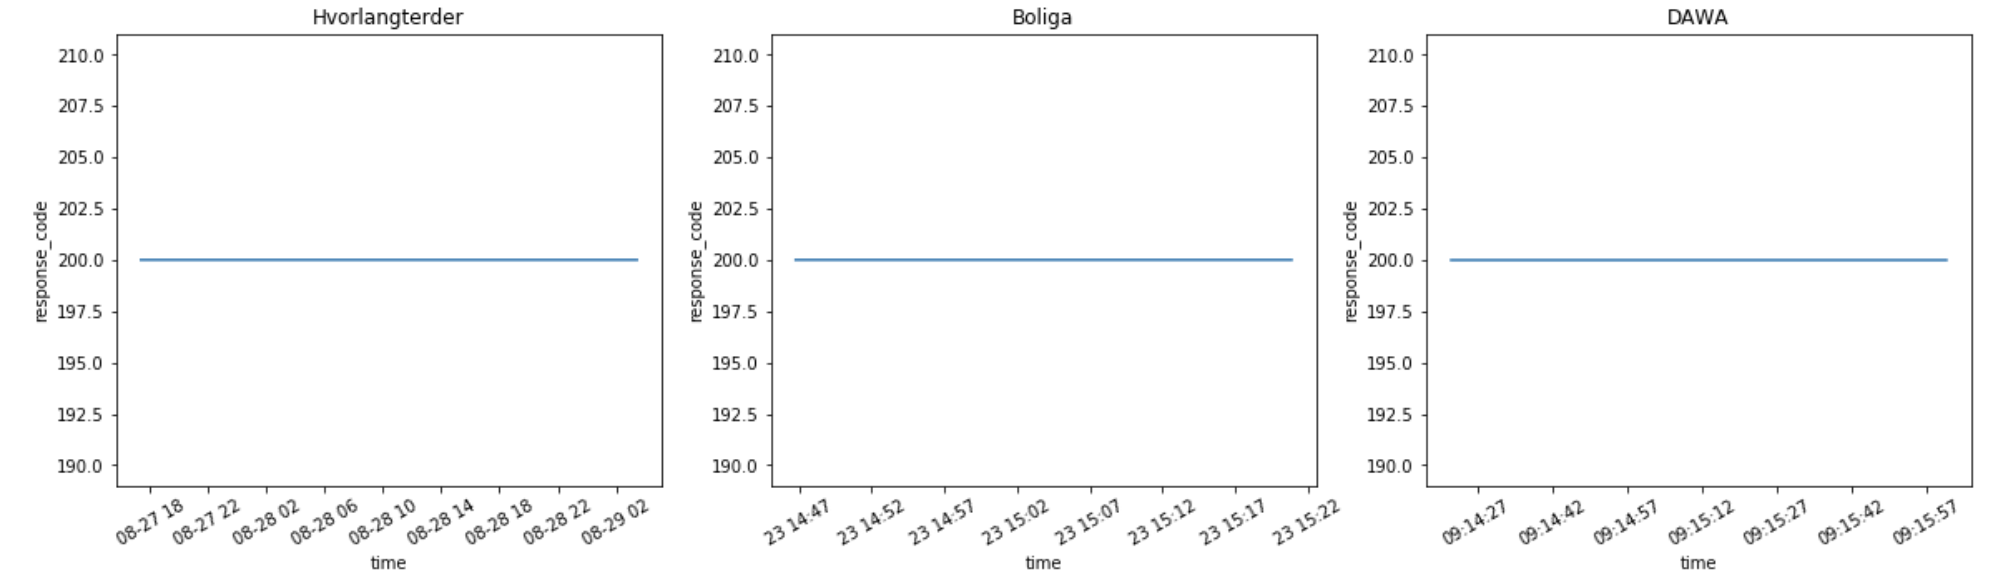
\includegraphics[width=\linewidth]{1log.png} 
  \label{fig:}
\end{figure}

\paragraph{Error Codes\newline}
Figure plots error codes received throughout the duration of the scrapings. Boliga and DAWA received no errors, while hvorlangterder received a total of 80 errors. The error code returned the same response in all 80 cases: \small{\textbf{('Connection aborted.', RemoteDisconnected('Remote end closed connection without response'))}}
\normalsize
\begin{figure}[H]
  \centering
   \caption{}
   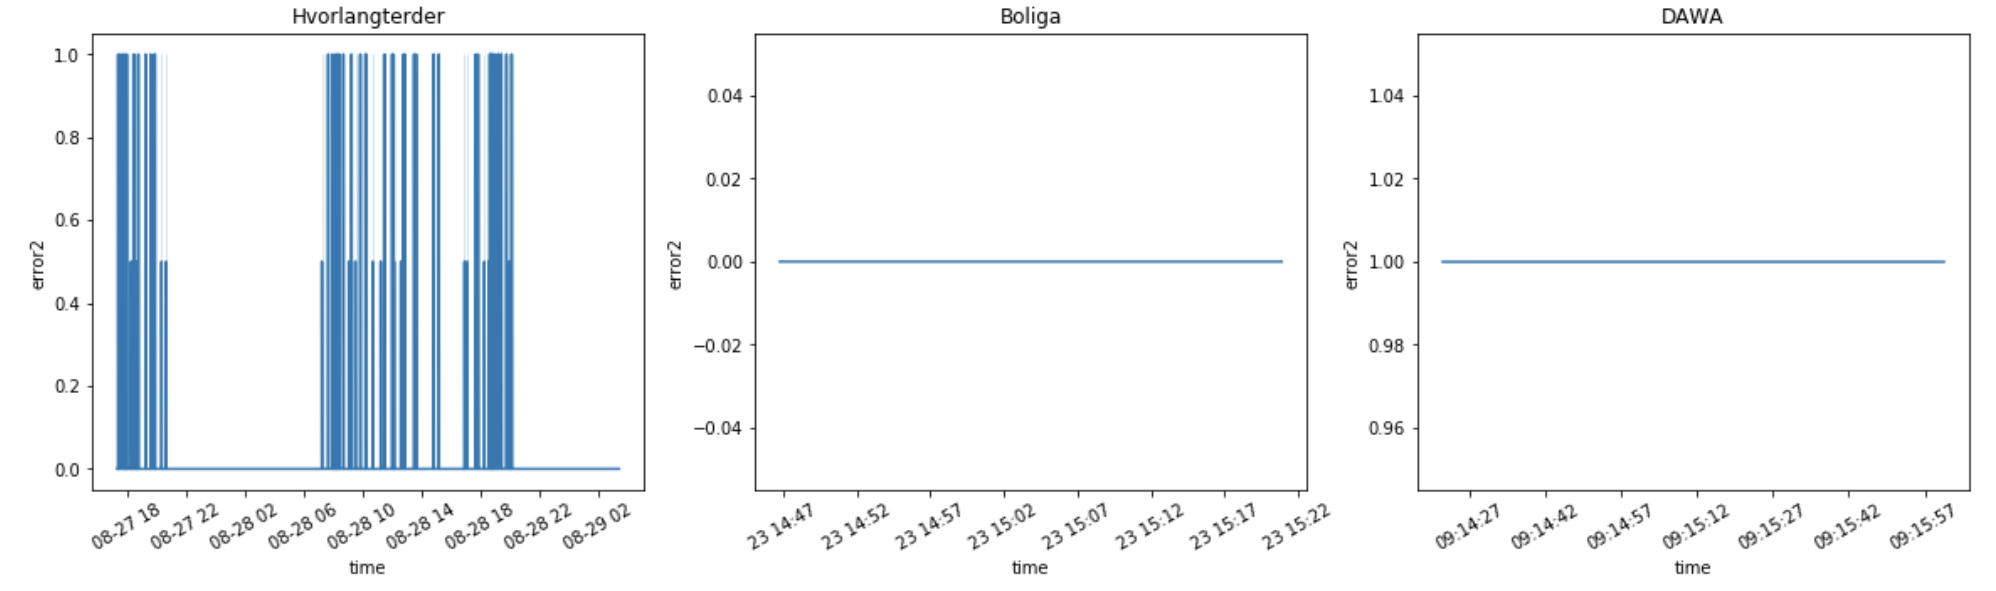
\includegraphics[width=\linewidth]{2log.png} 
  \label{fig:}
\end{figure}
To understand the errors, a closer manual analysis of the log was performed on requests receiving errors. The errors occurred in random intervals and were subsequently followed by another request to an identical URL. Therefore, we assessed that these errors were due to connection problems or server traffic. Since the errors were corrected by a following request, it should not affect the research.

\paragraph{Server Response Times\newline}
An indicator of poor data quality is varying response times from the server being scraped. \textcolor{red}{Figure XC} plots changes in response times for the duration of the web scrapings. The three data sources all resulted in few variations of response time. Unusual response times has been assessed within the logs, to be caused by either a slow server connection, or due to larger quantities of data being requested. To validate the quality of data, manual control of the returned results and the website results was performed, without notice of significant corruptions in the data utilised in the research.
\begin{figure}[H]
  \centering
   \caption{}
   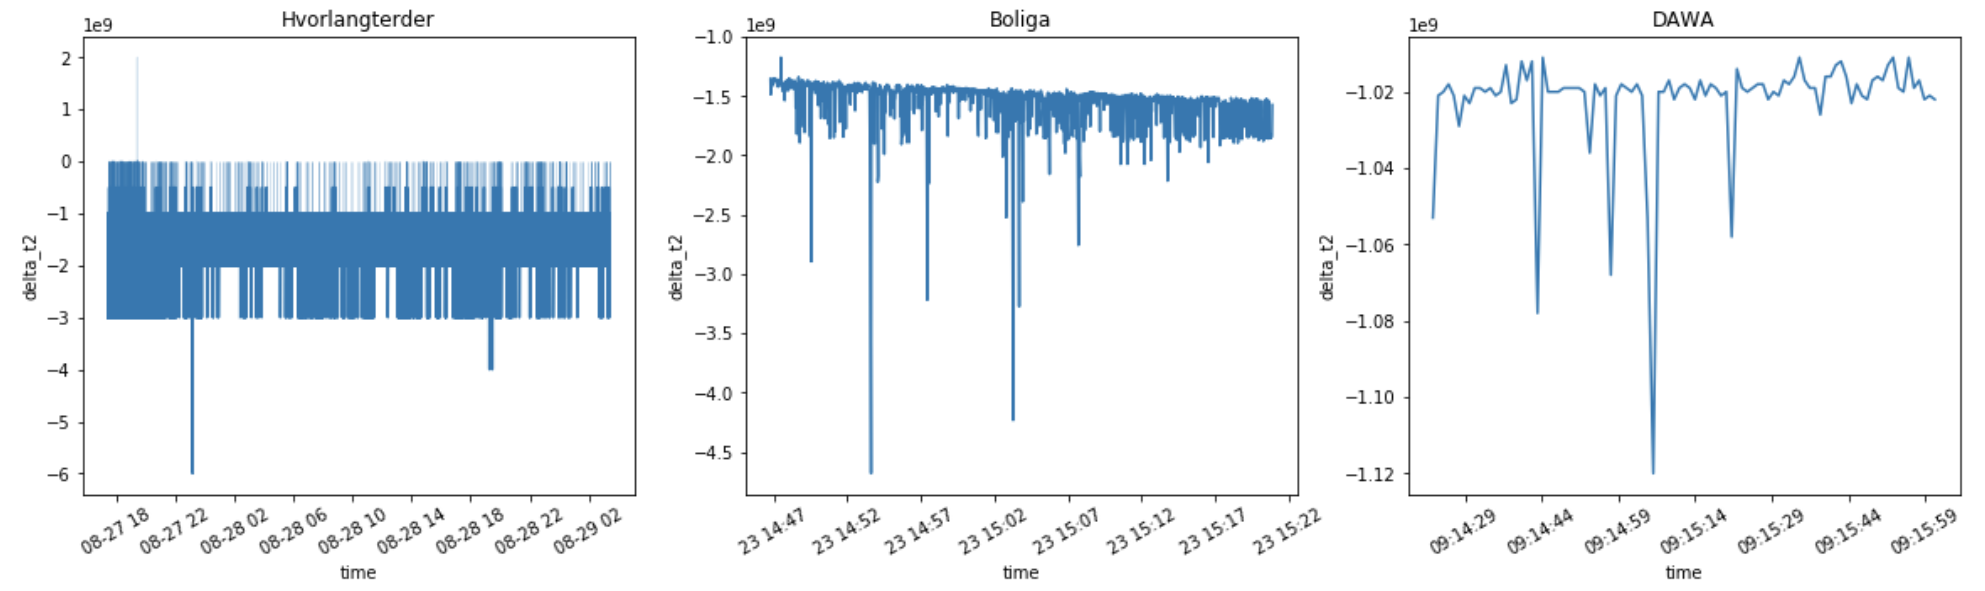
\includegraphics[width=\linewidth]{3log.png} 
  \label{fig:}
\end{figure}

\paragraph{Response Sizes\newline}
To validate the response quality, an assessment of the response size was performed. \textcolor{red}{Figure XD} plots response sizes throughout the duration of the web scrapings. Boliga contains a single noticeably large response size within short time, while hvorlangterder response sizes vary throughout the scrape. The DAWA scrape resulted in consistent response sizes, and therefore needed no further investigation. 
\begin{figure}[H]
  \centering
   \caption{}
   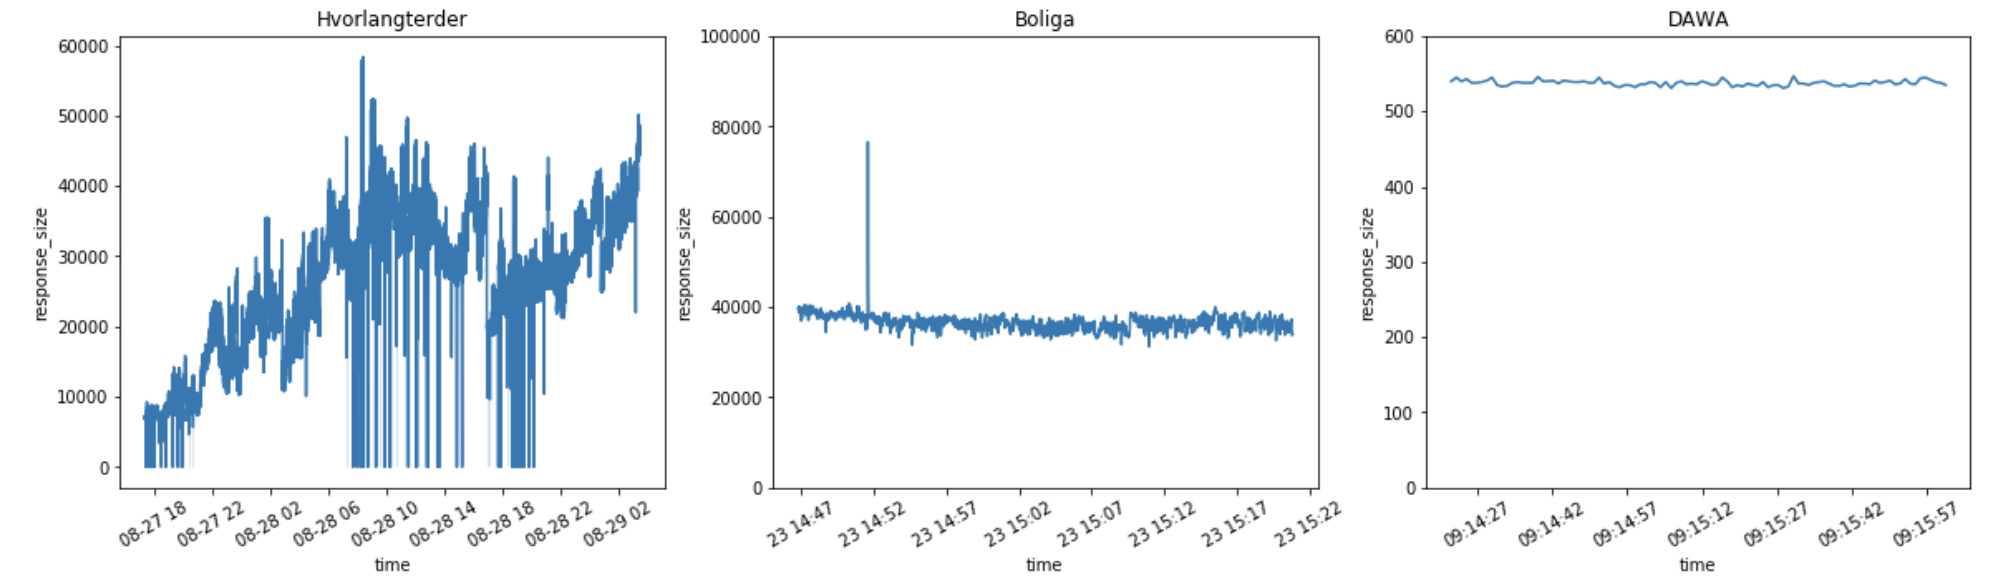
\includegraphics[width=\linewidth]{4log.png} 
  \label{fig:}
\end{figure}
Examining the distribution of sample sizes in figure XE, the Boliga and DAWA response sizes seem to be close to normally distributed, except for two single cases of large sample sizes in the Boliga log. By manually assessing the returned output of the Boliga scrape, these two requests were found to return a larger amount of data than usual. The requests were made to two pages, where a few properties contained nested dictionary attributes approximately 59 times larger than the average size of dictionaries within the ‘image’ data column. These dictionaries were image descriptions, and were not utilised within this research. These larger responses were deemed as not polluting the results of the research.
\begin{figure}[H]
  \centering
   \caption{}
   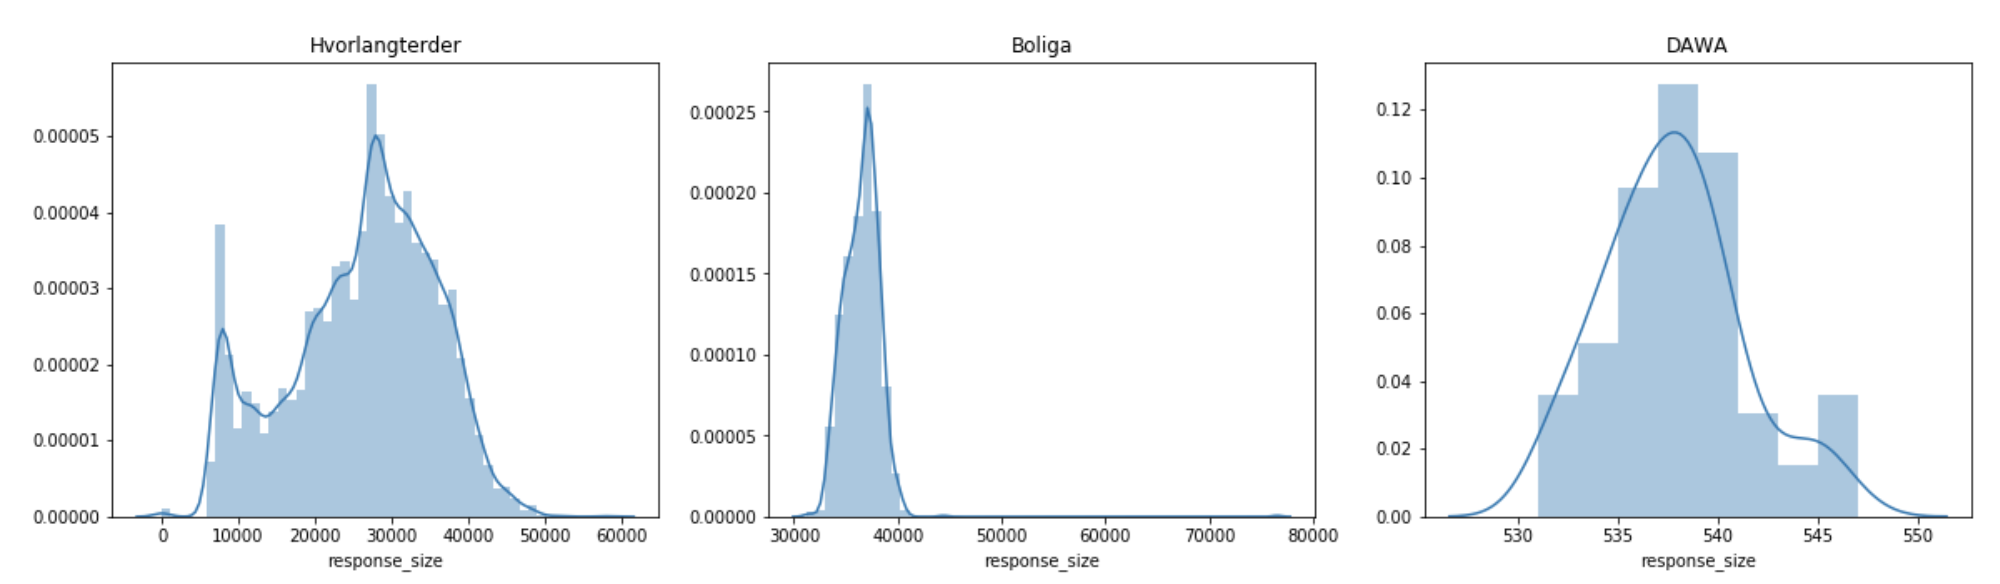
\includegraphics[width=\linewidth]{5log.png} 
  \label{fig:}
\end{figure}
\textcolor{red}{Figure XE depicts that the hvorlangerder response sizes were a bit left skewed, while Figure XD} shows that the distribution of large sizes happens during the middle of the scrape. With a further glimpse into the log, we observed two things. Firstly, all response sizes of 0 are related to the errors, displayed in figure XB. The variance of responses could be explained by the type of data retrieved from the scrape. The request was set to return names, addresses, distances and other information, which sizes are varying in nature. When extracting the value from every single key of the dictionary output, no errors or missing values were found. Further control of samples of large and small sizes was performed without discovering flaws. The response sizes from hvorlangterder are found to vary in nature, which may explain the difference.  

\paragraph{Assessment of the Scraping Logs\newline}
The individual analysis of the scraping logs showed minor suspicious traits which were assessed manually through the output or logs. The most noticeable analysis being differences in response sizes and response times from the hvorlangterder scrape. This scrape consumed large amounts of time and computing power, as every single observation from the Boliga data, had to be input for requesting a response. In an extensive research, these problems could be handled by gaining direct access to the website instead of scraping and would benefit from running on a server with greater computing power. The results of the data collection were evaluated to be satisfying, and not corrupting the results of our research, as fairly reasonable explanations for noticeable dissimilarities within the logs were found. 

\paragraph{Critique of Logs Using Scraping Class\newline}
In the process of analysing the scraping logs, minor flaws from the scraping library named ‘scraping\_class’ were detected. The returned columns ‘t’ and ‘delta\_t’ contained non-generic formats of epoch time. This was fixed by applying string manipulation and datetime conversions. 

\subsection{Merging Data}
Pandas objects can be combined in different ways according to the nature of the features in the dataset. Relational database style operations are based on linking keys together, thereby maintaining the relationship between the combined datasets\footnote{McKinney, W. (2018). \textit{Data Wrangling: Join, Combine and Reshape}. p. 231 }.

The data collection and scraping process provided a total of 15 Datasets from Boliga, Hvorlangterder, DAWA, the Danish Police, Social- \& Indenrigsministeriet and Danmarks Statistik. This section will describe how each dataset was merged, using pandas relational database styled merge and join operations. 

\paragraph{Boliga.dk\newline}
An evaluation of the Boliga datasets features and their ability to support further data collection led to the utilization of the following features: 

-	[Longitude, Latitude]: Geographical placements of the properties

-	Municipality: a numeric code for municipalities in Denmark

The Boliga dataset acted as a master dataset and was joined or merged upon throughout the process, and acted as the \textit{left} of all operations. The Longitude and Latitude features served as specific coordinates for valued properties but were in few cases repetitive regarding different apartments from the same complex. The municipality code was used for translational purposes between the master dataset and other datasets.  

\paragraph{DAWA\newline}
The DAWA dataset was scraped with an input of a distinct municipality code from the master dataset, returning a dataframe of municipality names for each code. This dataframe was merged onto the Boliga dataframe using a many-to-one merge with municipality codes as the merge keys. The scraped municipality names from DAWA was used as the merge key for all further merges of municipal data. 

\paragraph{Danmarks Statistik, Danish Police \& Social og Indenrigsministeriet\newline}
Of the municipality-based data collected, the merging of these to our master dataframe was subsequently performed identically. Every dataset contained a column for unique municipality names and values for the given feature of the dataset. A many-to-one left merge was performed with the master dataframe, using municipality names. The result being a master dataframe containing municipal specific features for properties. 

The Danish Police datasets contained totals for different categories of crimes reported within municipalities. These datasets were outer joined with an index set to contain municipality names. Afterwards, the values were added to each other, providing a total of reported crimes within each municipality. The police statistics website does not specify whether different types of reported crimes can relate to a single case, but we assessed that the number of crimes reported provides a meaningful feature either way. The dataset containing total reported crimes per municipality was merged with the master dataset in the same fashion as previous municipality-based features. 

\paragraph{Hvorlangterder.dk\newline}
The hvorlangterder scrape provided location specific features, taking an input of Latitude and Longitude coordinates. The scraping function, which was created for returning location-based features, created a column for the row specific values. Therefore, a merge operation was not necessary, but could alternatively have been managed with a one-to-one inner-merge on id. As few coordinates regarding apartment properties are repetitive, these are not suitable for merging upon. 

\subsection{Data Cleaning}
The scraping of Boliga left us with 65,950 observations. However, big data is often dirty and requires tidying before it can be used in any meaningful statistical context (Salganik 2018). The data cleaning process consists of removing duplicate values, handling missing data and manipulating strings\footnote{McKinney, W. (2018). 'Data Wrangling: Join, Combine and Reshape'. In W. McKinney, \textit{Python for Data Analysis} p. 191}. The pandas library contains functions to handle these data cleaning methods and was used throughout the process. In the following sections we describe our data cleaning efforts. 
\subsubsection{Initial clean-up}
The initial clean-up filtered out rows that contained illogical values. Here we focused our efforts on removing any and all observations that contained a municipality code of zero. Additionally, we chose to exclude any real estate valued below DKK 100, these listings existed on Boliga's website, but were all auction listings. We excluded these listings on the basis that they were unrealistically priced compared to the property's real market value.\newline
Boliga subdivides its listings into ten real estate types. We chose to exclude the typification "other", as there were only 17 houses listed in the category - too few for training our machine learning model. Furthermore, we also removed any listing without coordinates as these were vital for the scraping process of hvorlangterder.dk.\newline
We dropped all observations with an unreasonably high days-for-sale, as we saw these instances to not  represent reasonable pricing or demand. We have thus set an arbitrary limit of 3 years (1,095 days), and omitted any observations that has been on the market for longer than that. This results in the omission of approximately 5\% of our dataset. The highest mean "days-for-sale" on a municipal level was roughly 600 days, so to avoid discrimination against the observations from the municipalities with a longer average days-for-sale we set the cut-off somewhat higher than the highest mean. Another option was to set the limit according to each municipality's mean, a solution that was a bit more time consuming.
In figure XX the number of rows dropped at each step of the cleaning can be perused.
\begin{table}
\begin{center}
\caption{Filtered Rows\label{time}}
\begin{tabular}{|l|c|}
\hline 
\textbf{Feature} & \textbf{\emph{n}} \\
\hline 
Municipality code & 231 \\ 
\hline 
Price & 11 \\ 
\hline 
Coordinates & 275 \\ 
\hline 
Type & 17 \\ 
\hline 
days-for-sale & 3,940\\
\hline 
Total\tablefootnote{The total is the count of how many rows were dropped. Some rows were missing multiple features} & 4,332\\
\hline
\end{tabular} 

\end{center}
\end{table}
\subsubsection{Ejerlejlighed's lot size}
Inspecting our data we found that out of 8,028 apartments, 1,176 had a lot size. These listings included the apartment complex' common area, whereas the rest did not. To overcome this discrepancy we chose to set all non-zero values to zero, as not to confuse our model with an inconsistent feature (Raschka \& Mirjalili 2017).

\subsubsection{Final touches}
After merging the housing info with the demographic data and the distances from hvorlangterder.dk, we removed a single duplicate and deleted all columns not relevant for our analysis. After the clean-up of the data we were left with a dataset consisting of 61,618  observations, 37 features and 1 target variable. The features are of both categorical and continuous measures

\subsection{Descriptive Statistics}
In this section, we will examine the more apparent patterns of our collected data. This is done to familiarise ourselves with the data, before we commence the analysis.
\subsubsection{Key Statistics}
Some key statistical characteristics are presented in table 1:
\begin{table}[H]
\begin{center}
\caption{Key Statistics\label{time}}
\begin{tabular}{| c | c | c | c | c | c |} 
\hline
   & Price & \, Rooms \ & \ $m^2$ \ & Average Municipal Income \\ \hline
   Mean & 2,312,798 & \ 4.21 \  & \ 127.82 \ & 312,957.03 \\ \hline
   Std & 2,351,127 & 2.12 & 75.67 & 46,095.34 \\ \hline
   Min & 15,000 & 0 & 0 & 257,776 \\ \hline
   25\% & 985,000 & 3 & 82 & 290,973 \\ \hline
   50\% & 1,695,000 & 4 & 123 & 302,153 \\ \hline
   75\% & 2,895,000 & 5 & 167 & 318,745 \\ \hline
   Max & 85,000,000 & 50 & 2,390 & 583,331 \\ \hline
\end{tabular}
\end{center}
\end{table} 
Initially, it should be addressed that some of the properties has 0 rooms and consists of 0 $m^2$.  This is due to the fact that we have also included land on which housing has not yet been built. Examining the 25\%-quintile and the 75\%-quintile of the valuation prices, it becomes apparent that there are some substantial outliers both to the cheaper and to expensive side.


It is worth noting, that there is quite a big difference between the lowest average municipal income of DKK 257,776. and the highest of DKK 583,331. This difference becomes further noteworthy when assessing the 75\%-quintile. The difference from the 75\%-quintile to the highest average municipal income is more than 4 times the difference of the 75\%-quintile and the lowest income. The income distribution is visualised in the following figure:
\begin{figure}[H]
  \centering
   \caption{}
   \includegraphics[width=\linewidth]{Box1.png} 
  \label{fig:}
\end{figure}
The boxplot illustrates that the distribution is heavily left-skewed, where some municipalities has a sizebly higher average income than the rest of the Danish municipalities. 

\subsubsection{Prices in Municipalities}
We plot the average square meter valuation price in the different municipalities:
\begin{figure}[H]
  \centering
   \caption{}
   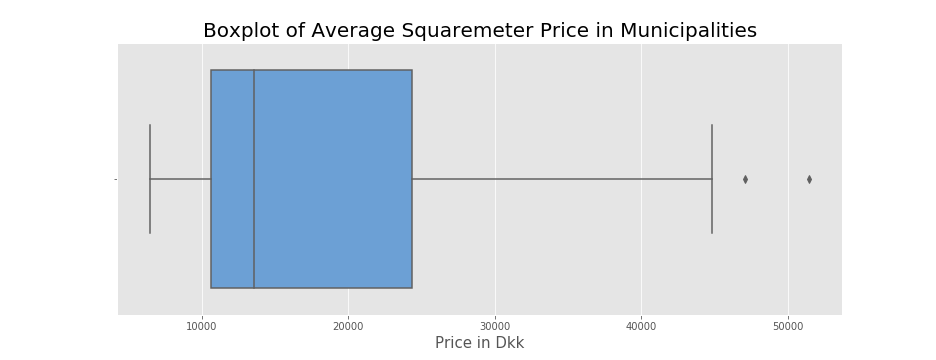
\includegraphics[width=\linewidth]{Box2.png} 
  \label{fig:}
\end{figure}
It becomes apparent that the distribution is quite right-skewed and that there are a few municipalities who’s price per square meter is much higher than the rest of the municipalities. Recalling the geoplot in figure 1, these expensive outliers are heavily concentrated around- and north of Copenhagen. 
The distribution looks similar to that of figure 2 (The previous boxplot), though we cannot declare any correlation between average municipal income and average municipal price per square meter. Nonetheless, it becomes apparent that the valuation price of property is highly discriminated by municipal factors. The scope of this assignment is exactly to examine these factors and attempt to use these to evaluate an unseen, out-of-sample property. 

\subsubsection{Property Type}
Another worthwhile consideration is that we have included all types of properties. It would be reasonable to assume that there is an average difference in valuation pricing depending on the type of property. Figure 4 displays the median valuation price for each type:
\begin{figure}[H]
  \centering
   \caption{}
   \includegraphics[width=\linewidth]{bar1.png} 
  \label{fig:}
\end{figure}
It is interesting to note that the most expensive properties are apartments as opposed to houses. This is not especially surprising though, as it is a well-established trend that real estate prices in major cities are skyrocketing. Refraining from delving deeper into a discussion of global urbanization, we retain the fact that property type does have an apparently significant effect on average valuation. We will include the ‘type’ feature in our impending model training to control for this effect. 


\section{Methods}
The objective of applying Machine Learning(ML) is to train a model that is able to make predictions on never seen data. By feeding a model labelled data as well as data samples, ML will define the algorithms that performs best predictions\footnote{Rashka, Sebastian; Mirjalli, Vahid; \textit{Python Machine Learning, Machine Learning and Deep Learning with Python, scikit-learn, and Tensorflow}. p. 3}. This project implements a ML regression prediction model.
\subsection{Fitting the model}
The potential problems of underfitting and overfitting should be assessed when fitting a model to data. A model is underfitted if it hardly captures the variation of the sample data. It is then said that the model has \textit{high bias}. A model is overfitted, when it is overly sensitive to the idiosyncrasy of the sample data and captures the variation in too great detail. This problem often comes with the introduction of a sizeable number of features. Overfit models are said to have \textit{high variance}\footnote{Rashka, Sebastian; Mirjalli, Vahid; \textit{Python Machine Learning, Machine Learning and Deep Learning with Python, scikit-learn, and Tensorflow}. p.73}. In both cases, the model will generalise poorly. A key step in defining a decent model in machine learning is to find an optimal bias-variance-balance, by tuning the complexity of one’s model. This is done through \textit{regularization}. In this project two different types of regularization are applied; LASSO and RIDGE.

\subsubsection{LASSO}
Regularization by LASSO, will penalise complexity of the model by the sum of the absolute value of the coefficients. This penalty will make the model less complex and more appropriate for prediction.  \footnote{Foster, Ian; Rayid Ghani Ron S. Jarmin, Frauke Kreuter, Julia Lane; \textit{Big Data in Social Sciences, A Practical Guide to Methods and Tools} p. 173}\, \footnote{Rashka, Sebastian; Mirjalli, Vahid; \textit{Python Machine Learning, Machine Learning and Deep Learning with Python, scikit-learn, and Tensorflow} p. 332}
\newline LASSO minimises: $$L_{LASSO}(\hat{\beta}) = \left(\sum_{i=1}^{n} (y_i-\hat{y_i}(\beta))^2+\lambda\sum_{j=1}^{p}|\hat{\beta_j}|\right) \qquad s.t \quad \lambda \geq 0 $$
Another convenient attribute of the LASSO penalty is that some estimates are set equal to zero and thereby produce sparse models\footnote{Hal R. Varian. \textit{Big data: New tricks for econometrics}. Journal of Economic Perspectives. p.19}. LASSO thereby performs feature selection automaticly.   
\subsubsection{RIDGE}
Opposed to LASSO, RIDGE does not force features to be omitted. Instead RIDGE penalises the magnitude of the coefficients. RIDGE minimises:
$$L_{RIDGE}(\hat{\beta}) = \left(\sum_{i=1}^{n} (y_i-\hat{y_i}(\beta))^2+\lambda\sum_{j=1}^{p}\hat{\beta_j}^2\right) \qquad s.t \quad \lambda \geq 0 $$ 

\subsection{Selecting Features}
In case regularization is not sufficient to cope with the overfitting of the model, exclusion of features is a viable approach. With the number of scraped features in this project taking into consideration, A recurring overfitting of the model would be likely. As a consequence a deliberate exclusion of features of interest are necessary.    

\subsection{Optimising the Hyperparameter}
To minimise the mean squared errors of our LASSO and RIDGE regression we performed k-fold cross validation to optimise the hyperparameter $\lambda$. 
We split the data into a test set and a development set, consisting of respectively 20\% and 80\% of the total observations. Subsequently, we use k-fold cross-validation to randomly split the development set into k folds, where k-1 folds are used to train the model. The remaining fold is used to validate the model’s generalizability by calculating the mean squared errors of the trained model’s prediction of the left-out fold\footnote{Rashka, Sebastian; Mirjalli, Vahid; \textit{Python Machine Learning, Machine Learning and Deep Learning with Python, scikit-learn, and Tensorflow}. p.191}. This process is repeated k times and each time a new fold is left out for validation. Since we are working with a relatively large dataset we chose to split our data into 5 folds, and computed the average MSE for the 5 iterations. By using the k-fold cross-validation method we minimise the concern that the estimation of our model’s performance is simply due to a lucky or unlucky split of the data. \newline
We performed this procedure for different values of $\lambda$. We chose the value of $\lambda$ which yielded the smallest average MSE over the 5 folds. 
We both calculated the optimal hyperparameters for a RIDGE regression model and a LASSO regression model.

\subsection{Predictive Performance}
With the hyperparameters optimised, final model performance can be evaluated. Once more a cross-validation is carried out, which returns the average performance error of each model. By retraining the models on the complete training set and testing on the independent test set, performance measures are obtained\footnote{Rashka, Sebastian; Mirjalli, Vahid; \textit{Python Machine Learning, Machine Learning and Deep Learning with Python, scikit-learn, and Tensorflow}. p.192}. \newline The performances of the models are simply measured by MSE and MAE. \newline
$$ MSE = \frac{1}{n}\sum_{i=1}^{n}(y_i-\hat{y_i})^2$$
$$ MAE = \frac{1}{n}\sum_{i=1}^{n}|y_i-\hat{y_i}|$$



\section{Analysis}
A number of features are excluded before training the model. The exclusion is determined, quite simply, by investigation of the correlation between the complete set of features and the target variable. A list of the excluded features is found in appendix 11.0.1. The model used for ML is found in appendix 11.0.2.  

The initial 5-fold cross-validation to obtain the optimal values of the hyperparameters in each regularization yields. 
\begin{table}[h!]
\begin{center}
\caption{Optimal hyperparameters, two degrees polynomial features\label{time}}
\begin{tabular}{ c | c  c  c } 
  & $\lambda_{LASSO}$ & $\lambda_{RIDGE}$ \\ \hline
2 degrees  & 372.76 & 26.83 \\ \hline
3 degrees  & 2310.13 & 432.88
\end{tabular}
\end{center}
\end{table} 

The prediction-errors of each model, with two and three degrees of polynomial features respectively, are printed below:
\begin{table}[H]
\begin{center}
\caption{Prediction Errors. \label{time}}
\begin{tabular}{| c | c | c | c | c | c |} 
\hline
   & \ MSE \ & \, RMSE \ & \ MAE \ \\ \hline
   LASSO 2-deg & 59,081,597,331.11 & \ 243,067.06 \  & \ 47,660.52 \ \\ 
  RIDGE 2-deg & 62,416,553,466.45 & 249,833.05 & 51,306.19  \\ 
  OLS 2-deg & 64,297,245,726.80 & 253,569.02 & 52,035.52  \\ \hline 
  LASSO 3-deg & 60,103,955,188.37 & 245,161.08 & 47,126.43  \\ 
  RIDGE 3-deg & 55,667,264,851.14 & 235,939.11 & 43,630.55  \\ 
  OLS 3-deg & 2.848e+28 & 1.68,7e+14 & 2.637e+12  \\ \hline
\end{tabular}
\end{center}
\end{table}
Since our efforts are aimed at predicting the valuation of a given real estate, we want to penalise the size of the error. Hence, the MSE-score is a better indicator for our model's performance as opposed to the mean absolute error (MAE). Since MSE squares the error terms, it gives a relatively high weight to large errors, which is desirable for our current aim. 

From table 4 it is evident that the model with 3 degrees of polynomial features regularised by RIDGE regression performs best. We are somewhat satisfied with the average performance of the model. With an MSE of approximately $55\cdot10^{10}$ and a MAE of DKK 43,630.55, we find that the model performs quite well on unseen data. Therefore, we chose this model as the final model from which we will conduct the rest of the analysis with. Assessment of the preferred model is conducted below. \newline


\paragraph{Learning Curve\newline}
We examine the learning curve of the model to assert whether the model suffers from immediate over- or underfitting problems and whether these would be remedied by collecting more data\footnote{Rashka, Sebastian; Mirjalli, Vahid; \textit{Python Machine Learning, Machine Learning and Deep Learning with Python, scikit-learn, and Tensorflow} p. 196}
The following plot illustrates the learning curve of our model:
\begin{figure}[H]
\centering
\caption{}
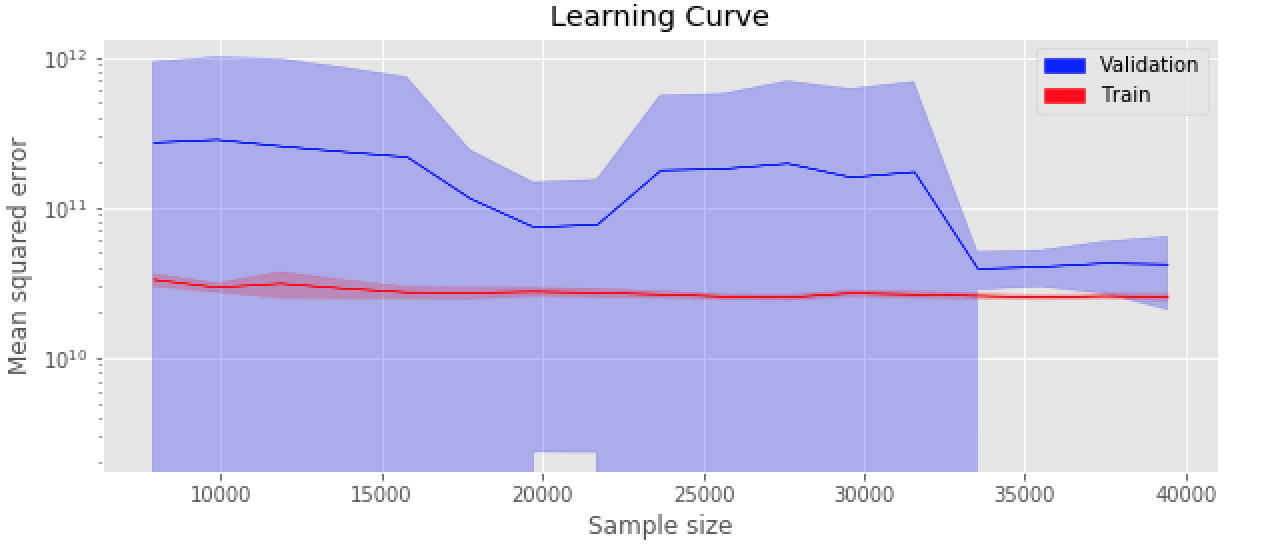
\includegraphics[scale=0.6]{Learncurvridge.png}
%\source{}
\end{figure}
The plotted curves represent the average performance of the validation- and training sets, while the width of the plotted curves expresses the 95\%-confidence interval of the performance.  
The performances on the validation set are very inconsistent and varies a lot. None the less, it seems as if the gap is decreasing between the performances of the training- and validation sets as the sample size increases. 
At around 33,000 observations the validation curve drastically decreases and both curves flatten out. Though the confidence interval of the validation performance is still noteworthy, it also improves dramatically when the sample gets sufficiently high. Just before 40,000 observations, the confidence interval of the validation curve actually drops below the train curve, which should not be possible. We have not found a meaningful explanation aside from noise or chance \footnote{\href{https://jakevdp.github.io/PythonDataScienceHandbook/05.03-hyperparameters-and-model-validation.html}{jakevdp.github.io/PythonDataScienceHandbook/05.03-hyperparameters-and-model-validation.html}} 
All in all, the learning curve would indicate that the performance of the model will not benefit from additional training data. 

\paragraph{Validation Curve\newline}
We examine the validation curve of the model to see whether we have found a good bias-variance trade-off with our optimised hyperparameter. We plot the average train and cross-validation performance for different values of $\lambda$: 
\begin{figure}[H]
\centering
\caption{}
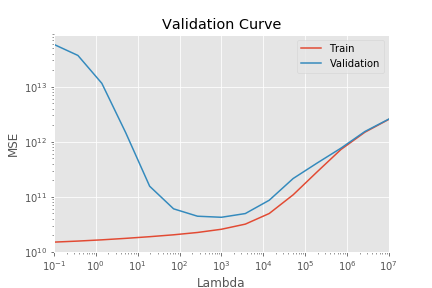
\includegraphics[scale=0.6]{ValCurveRidge3deg.png}
%\source{}
\end{figure}
The dotted line approximately represents the optimised value of lambda from our previously conducted k-fold cross-validation. 


The curves suggest that we have found the optimal degree of regularization with our hyperparameter. Had we chosen a smaller value of $\lambda$, the model would have had too high variance and thus been overfit. This is deduced by how poorly the validation predictions performs at smaller $\lambda$, as opposed to the training performance. On the contrary, had we chosen a greater value of $\lambda$, the model would have been too biased. This is illustrated by how poorly the training data, as well as the validation data, performs at higher values of $\lambda$ . In that case, we would have underfitted our model. 
Nonetheless, it is apparent that our model performs better on the training data, which indicates that it retains a degree of overfitting. For the abovementioned reasons, it would not be meaningful to minimise this performance gab by adjusting the hyperparameter. Other options for decreasing the variance of the model, could be to include more training data, but as illustrated by the learning curve, this would not seem to effect the variance. Lastly, as overfitting is often caused by a sizeable number of features, omission would be a reasonable mean. As we have already conducted feature selection on the basis of correlations, we did not find a feasible way to conduct further selection without omitting theoretically warranted features. This could be a subject for further studies, to investigate whether this could improve the performance and evaluation of the model. \newline
To sum up it would seem that we have found the hyperparameter which yields the optimal bias-variance trade-off. We can thus conclude that we have optimised our model under the given resources. 

\section{Discussion}
\subsection{No Grid Search or One-to-many}
$$L_{elasticnet}(\hat{\beta}) = \frac{\sum_{i=1}^{n}\left(y_i-\hat{y_i}(\beta)\right)^2}{2n} + \lambda\left(\frac{1-\alpha}{2}\sum_{j=1}^{p}\hat{\beta_j}^2+\alpha\sum_{j=1}^{p}|\hat{\beta_j}|\right)$$
$$0 \leq \alpha \leq 1 \quad \wedge \quad \lambda \geq 0$$

\subsection{Best Subset Feature Selection}
\subsection{Data critique}
An interesting prediction which could have been done using the same methods, would have been to predict selling prices. This could have been done simply by scraping data on sold housing. This could be of more value for private agents, whose main interest would be the actual selling price instead of the valuation. \newline 
In a prediction-model like this it is near impossible to evade some form of omitted variable bias. A significant amount of potentially important factors can not be acquired. For example the view from the listed housing will for sure be of great impact of the valuation price. Another factor of interest could have been an evaluation of the condition of the housing. Unfortunately the statement of property\footnote{red. Tilstandsrapport} are not publicly accessible. \newline
The prediction of the cooperative housing valuation %\footnote{http://housingpeople.dk/en/housing-guide/housing-types/cooperative-andelsbolig/},
are subject to significant bias, since the cooperative housing that enters the market through a realtor often would be those with critical amount of undesirable characteristics. Future studies could exclude cooperative housing in an effort to increase the prediction capabilities.  

\subsection{Model Limitations}
The exclusion of municipality dummies as regressors in the prediction models, leaves the model to only separate municipalities by the socio-economic factors, which are subject to low variance. This makes distinction between municipalities a lot more difficult as well as uncertain.   
Without the municipality dummies, the interpretation of the prediction results are more insecure. %Instead of predicting the valuation of a given estate, of a given type, in a given municipality or city. It predicts the valuation of a estate at a \textit{more or less} location in Denmark by type, only geographically controlled by distances to various conveniences. 
Geographical boundaries could have been limited way more, resulting in easier interpretation of predictions. Potentially by predicting only for a specific city or municipality. \\
If one intended to predict valuations country-wide more realisticly, a model for each municipality could have been more satisfactory, resulting in 98 separate models. The evident downside of this approach being the prospect of limitations in available data since some municipalities has very few listings.     
Another approach could have been to group cities which share characteristics. Ex. The three biggest cities, the islands, the country-side towns.    

\subsection{Model Selection}
Instead of only assessing the different models by MSE,
the information criteria of the respective models could have been introduced, which could have altered the selection of preferred model. Both AIC and BIC would likely have suggested LASSO with 2-degrees of polynomial features as preferred model, as both criteria are increasing with the numbers of estimated parameters\footnote{Peckov, Aleksandar. (2012)  \textit{A Machine Learning Approach To Polynomial Regression}}. 

\section{Conclusion}
In this assignment, we have used machine learning to train a model to predict valuation prices of real estate in Denmark. We did this by scraping Boliga.dk for all of their listed housing and combining this with municipal data on income, education, schools and urbanization. Additionally, we also scraped data from hvorlangterder.dk which calculates the distance from an address, to different every-day commodities such as hospitals, schools and shopping. 
We have explained how we carried out our gathering of data, how we have structured the data and how we cleaned it. \newline
We performed descriptive statistics to gain a better acquaintance with the data. 
We conducted feature selection by assessing the correlation between the different features and the target variable, which in our assignment has been the valuation price. 
We trained both a LASSO- and a RIDGE regression model and compared their performances with the performance of a standard linear regression. Through k-fold cross-validation, we estimated the optimised hyperparameters for both regularization models. We found that the RIDGE regression with three polynomial features performed best, at predicting out of sample data with the performance measure being the smallest mean square error. When predicting the test data the model had a MSE of 5.566e+10 with a optimised hyperparameter $\lambda$=432.88 which we found to be a decent performance. 
We have assessed the final model and examined to which degree we have managed to find a good bias-variance-balance for our model and concluded that our model suffers from a degree of overfitting. This was done by examining the validation- and learning curve of our final model. Additionally we addressed possibilities of further optimising the model.  \newline
Finally, we have discussed the results of our analysis. We have critically assessed the boundaries of our research and drawn up potential possibilities for improvement. 



\newpage
\section{Litterature}
\ Foster, Ian; Rayid Ghani Ron S. Jarmin, Frauke Kreuter, Julia Lane; \textit{Big Data in Social Sciences, A Practical Guide to Methods and Tools}, CRS Press 2017 \newline

Rashka, Sebastian; Mirjalli, Vahid; \textit{Python Machine Learning, Machine Learning and Deep Learning with Python, scikit-learn, and Tensorflow}, $2^{nd}$editon, Packt Publishing 2017. \newline

Varian. Hal R. \textit{Big data: New tricks for econometrics}. Journal of Economic Perspectives, 28(2):3–28, 2014. \newline

Consumer Data Research Center, UK  [CDRC] (2018) \textit{The General Data Protection Regulation \& Social Science Research} [Online]: \href{https://ec.europa.eu/research/participants/data/ref/h2020/other/hi/h2020_ethics-soc-science-humanities_en.pdf}{ec.europa.eu/research/participants/data/ref/h2020/other/hi/h2020\_ethics-soc-science-humanities\_en.pdf} [Accessed on 25/08/2019]\newline

European Commission (2018). \textit{Ethics in Social Sciences and the Humanities} [Online]: \href{https://ec.europa.eu/research/participants/data/ref/h2020/other/hi/h2020_ethics-soc-science-humanities_en.pdf}{https://ec.europa.eu/research/participants/data/ref/h2020/other/hi/h2020\_ethics-soc-science-humanities\_en.pdf} [Accessed on 25/08/2019] \newline

Popper, Karl (1969) \textit{The Moral Responsibility of the Scientist}. Encounter, March 1969, pp. 52-56 [Online]: \href{http://www.unz.com/print/Encounter-1969mar-00052}{http://www.unz.com/print/Encounter-1969mar-00052} [Accessed on 25/08/2019]\newline

Rotblat, Joseph (1999) \textit{A Hippocratic Oath for Scientists}. Science, November 1999: Vol. 286, Issue 5444, pp. 1475 [Online]: \href{https://science.sciencemag.org/content/286/5444/1475.full}{https://science.sciencemag.org/content/286/5444/1475.full} [Accessed on 25/08/2019] DOI: 10.1126/science.286.5444.1475 \newline
 
Salganik, Matthew J. (2018) \textit{Bit by Bit Bit - Social research in the digital age.} Princeton, NJ: Princeton University Press.\newline

Sample, Ian (2019, Fri 16 Aug 2019) \textit{and tech specialists need Hippocratic oath, says academic.} The Guardian [Online]: \href{https://www.theguardian.com/science/2019/aug/16/mathematicians-need-doctor-style-hippocratic-oath-says-academic-hannah-fry} [Accessed on 25/08/2019]\newline

Vox.com (2018) \textit{The Cambridge Analytica Facebook scandal} [Online]: \href{https://www.vox.com/2018/4/10/17207394/cambridge-analytica-facebook-zuckerberg-trump-privacy-scandal} [Accessed on 26/08/2019] \newline
 
Boligagruppen.dk (2019) \textit{Om boliga gruppen} [Online]: \href{https://www.boligagruppen.dk}{www.boligagruppen.dk}: [Accessed on 27/08/2019] \newline

Shiab, Nael (2015) \textit{On the Ethics of Web Scraping and Data Journalism. Global Investigative Journalism Network.} [Online]: \href{https://gijn.org/2015/08/12/on-the-ethics-of-web-scraping-and-data-journalism/}{gijn.org/2015/08/12/on-the-ethics-of-web-scraping-and-data-journalism/}: [Accessed on 27/08/2019] \newline

McKinney, W. (2018). 'Data Wrangling: Join, Combine and Reshape'. In W. McKinney, \textit{Python for Data Analysis}. Sebastopol: O'Reilly Media Inc. \newline

Athey, Susan (2018) 'The Impact of Machine Learning on Economics' in Ajay Agrawal et al. (eds) \textit{The Economics of Artificial Intelligence: An Agenda} (2019). Chicago: University of Chicago Press. \newline

Einav, Liran and Jonathan Levin (2014) \textit{Economics in the age of big data}. Science, vol. 346, November. \newline

Grimmer, Justin (2015) \textit{We are all social scientists now: how big data, machine learning, and causal inference work together}. PS: Political Science \& Politics, vol. 48, January: 80-83. \newline

Lazer, David and Jason Radford (2017) \textit{Data ex Machina. Introduction to Big Data. Annual Review of Sociology}, vol. 43, August. \newline

Mullainathan, Sendhil, and Jann Spiess (2017) \textit{Machine Learning: An Applied Econometric Approach}. Journal of Economic Perspectives, vol. 31 (2): 87-106. \newline

Anderson, Chris (2008) \textit{The end of theory: The data deluge makes the scientific method obsolete}. Wired, 16-07 [Online] \href{https://www.wired.com/2008/06/pb-theory/}{www.wired.com/2008/06/pb-theory/} [Accessed on 27/08/2019]\newline

Peckov, Aleksandar. (2012)  \textit{A Machine Learning Approach To Polynomial Regression}. Available at \href{http://kt.ijs.si/theses/phd_aleksandar_peckov.pdf}{kt.ijs.si/theses/phd\_aleksandar\_peckov.pdf}. Doctoral Dissertation. Jozef Stefan International Postgraduate School. Ljubljana, Slovenia, October 2012. [Accessed on 29/08/2019]

(https://jakevdp.github.io/PythonDataScienceHandbook/05.03-hyperparameters-and-model-validation.html). [Accessed on 29/08/2019]\newline

https://www.dst.dk/da/Statistik/nyt/NytHtml?cid=27979 [Accessed 27/08/2019]\newline

https://www.dst.dk/da/Statistik/nyt/NytHtml?cid=28741 [Accessed 27/08/2019]\newline
\newpage
\section{Appendix}
\subsubsection{}
Excluded Features:\newline
municipality, lotSize, unemployment, Total\_reported\_crime, Socioeconomic\_index, expenses\_per\_school\_student, expenses\_sport\_and\_other\_cultural\_activities, forest\_distance, coast\_distance, isForeclosure, owners\_expense
\subsubsection{}
The model used for prediction: 
$$ \hat{Y_i}=\hat{\beta_0}+\sum_{i=1}^p\hat{\beta_i}\textbf{T}_i+\hat{\epsilon_i},\quad T_i=\prod_{j=i}^pX_j^{d_i,j}
\quad\footnote{Peckov, Aleksandar. \textit{A Machine Learning Approach To Polynomial Regression} p. 6-9}$$
\small{$p$ being total number of features, $d_i,j$ denoting degree of polynomial features. 
$$\textbf{X}_j=\begin{bmatrix}
           basementSize \\
           buildYear \\
           rooms \\
           size \\
           primary\_school\_educ \\
           high\_school\_educ \\
           vocational\_educ \\
           SHE \\
           MHE \\
           bachelors\_degree \\
           LHE \\
           avg\_municipal\_income\_2017 \\
           Population\_in\_urban\_development \\
           Socioeconomic\_index \\
           lake\_distance\\
           doctor\_distance \\
           supermarket\_distance \\
           school\_distance \\
           daycare\_distance \\
           hospital\_distance \\
           train\_distance \\
           pharmacy\_distance \\
           library\_distance \\
         \end{bmatrix}$$
\end{document}